\documentclass[14pt]{extreport}

\usepackage{setspace}
\usepackage{graphicx}
\graphicspath{{./figures/}}


\begin{document}

\title{NightyBird\\Your Stay-up Assistent}
\doublespacing

\author{Yuefeng Zhou\\Xuping Lei}
\date{May 2, 2014}

\begin{titlepage}
    \centering
    \vfill
    {\bfseries\Large
        Nighty Bird\\
        Your Stay-up-late Assistance\\
        \vskip2cm
        Yuefeng Zhou\\
        Xuping Lei
    }    
    \vfill
    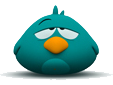
\includegraphics[width=7cm]{icon.png} % also works with logo.pdf
    \vfill
    \vfill
\end{titlepage}

\chapter{Overview}
NightyBird is an application for people to adjust their sleeping habits. It will remind user to go to bed when the user is staying up. It generates reports to give user advices on sleeping, sports and diets.

Users can check in when he is going to sleep or when he wakes up. The application will record that time for the users. Users can also input or edit his sleeping data manually. NightyBird provides users several interfaces to manipulate his sleep data. 

When the user is staying up very late, NightyBird will send notifications to the user to urge him to sleep. They "stay up late" is defined by the user. The user can also set up the period of notifications when staying up.

Users can view a daily report or a weekly report. The weekly report contains a range chart that makes it look more intuitive. In addition to the range chart, some suggestions are also included like sports advices or diet advices. These suggestions are fetched by a web service. The NightyBird application send user's sleep data to our server, the server responses with these suggestions.


\chapter{User Interfaces}

\chapter{Database}

\chapter{Entities}

\chapter{Report Web Service}

\chapter{Other Features}

\end{document}